\begin{frame}[fragile]{Framework overview}
\vspace{0.1cm}
    \begin{minipage}[h]{0.45\textwidth}
		\only<1>{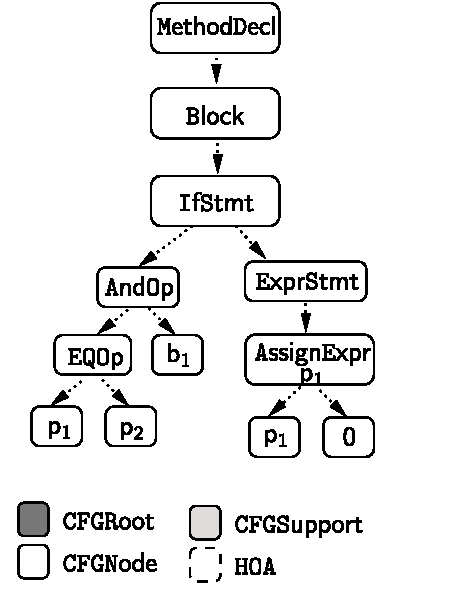
\includegraphics[scale=0.65]{img/framework1.pdf} }%
		\only<2>{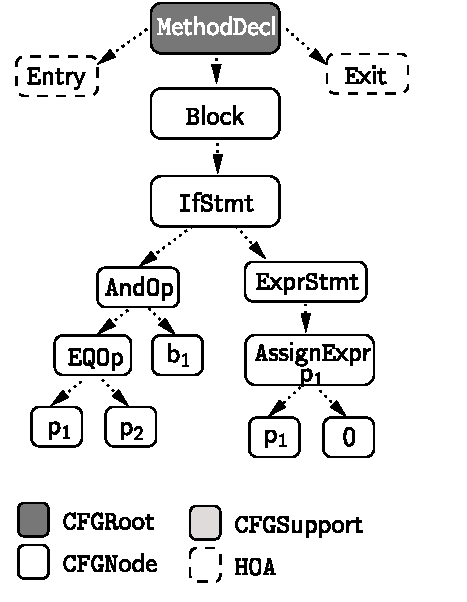
\includegraphics[scale=0.65]{img/framework2.pdf} }%
		\only<3>{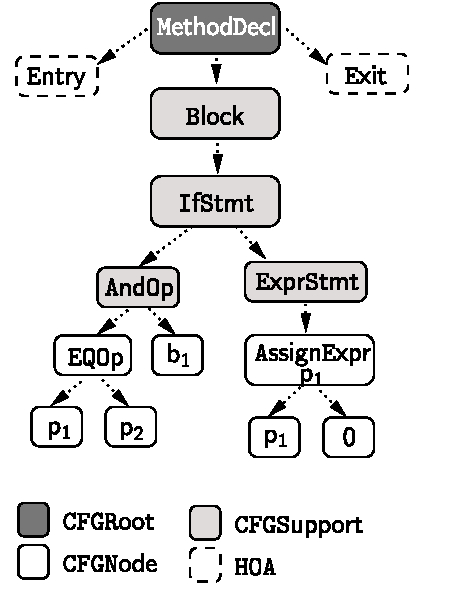
\includegraphics[scale=0.65]{img/framework3.pdf} }%
		\only<4>{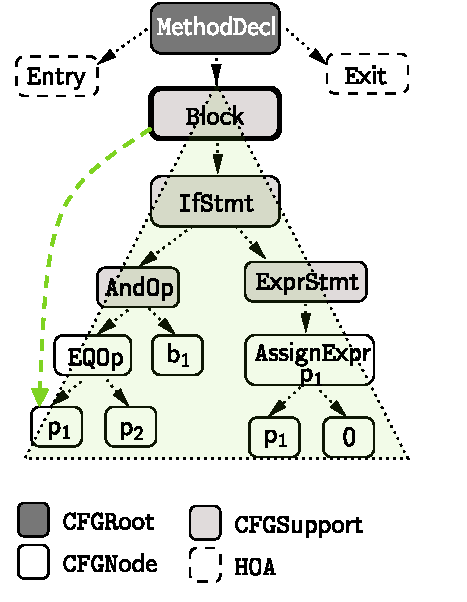
\includegraphics[scale=0.65]{img/framework3_1.pdf} }%
		\only<5>{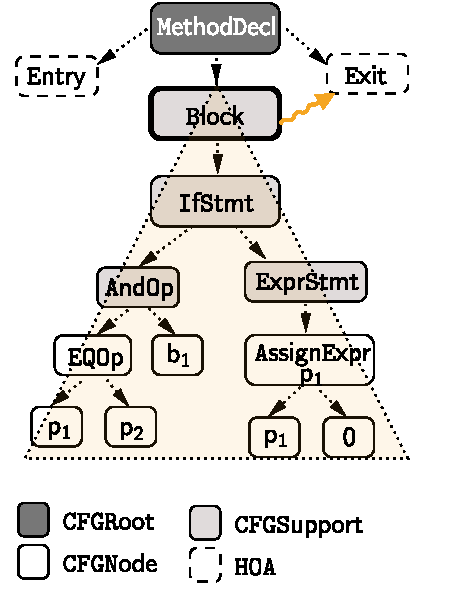
\includegraphics[scale=0.65]{img/framework3_2.pdf} }%
		\only<6>{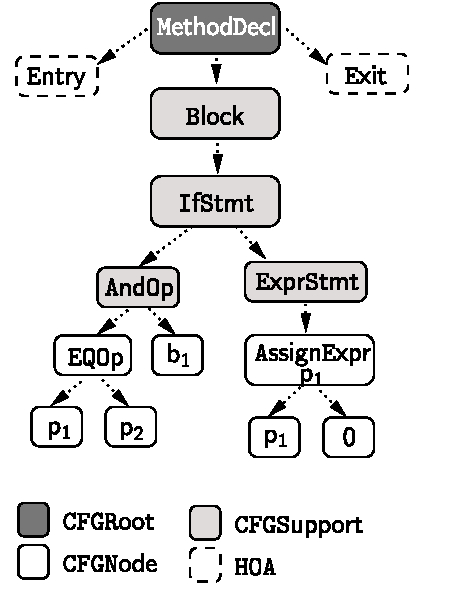
\includegraphics[scale=0.65]{img/framework3.pdf} }%
		\only<7>{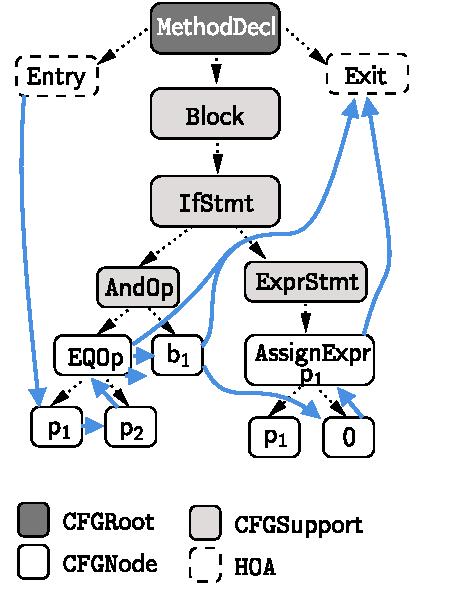
\includegraphics[scale=0.65]{img/framework4.pdf} }%
		\only<8>{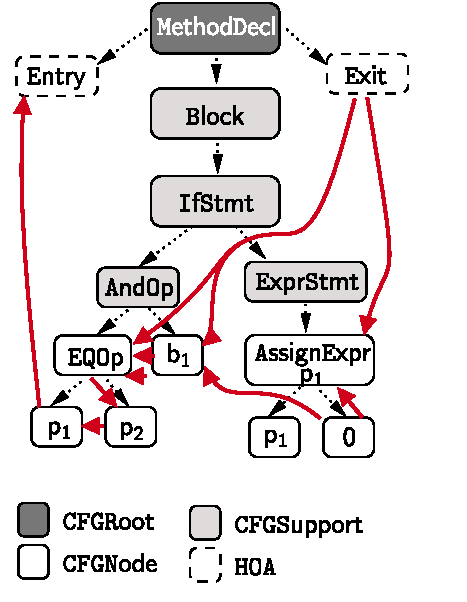
\includegraphics[scale=0.65]{img/framework5.pdf} }%
    \end{minipage}%
	\begin{minipage}[h]{0.6\textwidth}%
	\small
		  \begin{itemize}%
			\item<2-> \texttt{CFGRoot} extends the AST with two HOAs: \texttt{Entry} and \texttt{Exit}
			\item<3-> \texttt{CFGSupport} defines:
		\begin{itemize}
				\item<4-> \texttt{firstNodes}
				\item<5-> \texttt{nextNodes}
		\end{itemize}
			\item<6-> All the \texttt{CFGNode} are \texttt{CFGSupport}
%			\item \texttt{CFGNode} are the only with \texttt{succ} and \texttt{pred}
			\item<7-> Used \texttt{firstNodes} and \texttt{nextNodes} to compute the \texttt{succ} attribute
			\item<8-> The \texttt{pred} is computed as the inverse of \texttt{succ}
 		\end{itemize}%
\begin{lstlisting}[language=JastAdd]
foo(int p1, int p2, Boolean b1){
  if(p1==p2 && b1)
    p1 = 0;
}
\end{lstlisting}
    \end{minipage}%
\end{frame}



\begin{frame}{Challenges}
\begin{itemize}[<+->]
	\item We used HOAs to extend the AST with new subtrees
    \begin{minipage}[h]{0.6\textwidth}
    \begin{multicols}{2}
		\begin{itemize}
			\item Call to \texttt{close()} for resources in \textbf{Try With Resources}
			\item \textbf{Static} and \textbf{Instance}  initializers
			\item Exception-sensitivity by reifying  \textbf{Finally Blocks}.
			\item  Implicit condition in empty \textbf{For loops}
		\end{itemize}
	\end{multicols}%
\end{minipage}
	   \begin{minipage}[h]{0.3\textwidth}%
	     \onslide<5->{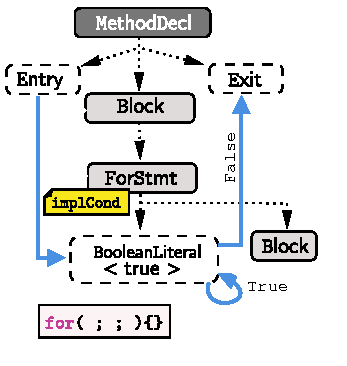
\includegraphics[scale=0.6]{img/ForExample.pdf}}%
    \end{minipage}%
	\item We used Circular attribute to compute mutually depended attributes
	\begin{itemize}
\item The attribute may depends on its own value
\item Computes a fixpoint
\end{itemize}
\end{itemize}
\end{frame}
